%%%%%%%%%%%%%%%%%%%%%%%%%%%%%%%%%%%%%%%%%%%%%%%%%%%%%%%%%%%%%%%%%
% Tese de Doutorado / Dept. Fisica, CFM, UFSC                   %
% Lacerda@CórregoGrande - Jan/2018                              %
%%%%%%%%%%%%%%%%%%%%%%%%%%%%%%%%%%%%%%%%%%%%%%%%%%%%%%%%%%%%%%%%%

%:::::::::::::::::::::::::::::::::::::::::::::::::::::::::::::::%
%                                                               %
%                      Anexo neb vs syn                         %
%                                                               %
%:::::::::::::::::::::::::::::::::::::::::::::::::::::::::::::::%

\chapter{Comparações entre propriedades estelares e propriedades nebulares}
\label{apendice:synvsneb}

Inicio este apêndice dizendo que esse ensaio foi feito antes do artigo \citet{Lacerda.etal.2018} e por isso engloba uma amostra diferente escolhida com outros objetivos, porém, por ser um estudo de grande importância, vale seu detalhamento nesta tese.

As propriedades da síntese são relacionadas às populações estelares e comparações com as nebulares podem nos ajudar a entender melhor a história de formação estelar de cada região. Durante os últimos anos esses estudos cruzados entre propriedades sintéticas e nebulares de quase um milhão de galáxias do \SDSS renderam ótimos resultados para o GAS-UFSC. Neste Apêndice faço uso do \emldc e do PyCASSO para comparar a taxa de formação estelar e o coeficiente de extinção por poeira, estimados através de linhas de emissão e da síntese. Esses experimentos foram executados também, em um formato mais completo, porém com dados de espectroscopia integrada do \SDSS, em \citet{Mari2016}.


\section{Ensaio}
\label{apendice:synvsneb:ensaio}
Um programa feito da união entre o PyCASSO e o EmLineDataCube nos instiga a comparar medidas nebulares com as propriedades estelares. O gás é o combustível da formação estelar. As nuvens de gás molecular, formadas pelo esfriamento de gás do meio interestelar, se fragmentam formando estruturas menores e cada vez mais densas. A formação estelar acontece quando o centro dessas massas de gás colapsam devido ao desbalanceamento entre pressão e gravidade.

% {\ATR MV DE LUGAR?? \ojo Essas regiões, que podem ser pequenas ou se estenderem a gigantes berçários estelares, estão geralmente cobertas por uma densa camada de poeira. No final do ciclo de vida das estrelas, diversos elementos são jogados no meio interestelar através das explosões de supernovas, alterando assim a composição química do gás disponível para produção de novas estrelas.
% }
%
%
% \citet{Schmidt.1959a} foi o primeiro a propor a existência de uma lei de potências que liga a taxa de formação estelar ({\em star formation rate}; SFR) e o gás. Anos depois, \citet{Kennicutt.1998a} estuda essa relação observacionalmente, utilizando diversos indicadores de formação estelar em diferentes faixas espectrais. Em seu trabalho, Kennicutt estabelece a ligação entre a densidade superficial do gás e da SFR. Hoje em dia essa é comumente chamada de relação de Kennicutt-Schmidt (KS) ou lei de formação estelar. A
% equação parametrizada por \citeauthor{Kennicutt.1998a} foi:
% \begin{equation}
% 	\Sigma_{\mathrm{SFR}}\ =\ (2.5\pm0.7)\times 10^{-4} \left(\frac{\Sigma_{\mathrm{gas}}}{
% M_\odot\ \mathrm{pc}^{-2}}\right)^{1.4 \pm 0.15}\ M_\odot\ \mathrm{yr}^{-1}\ \mathrm{kpc}^{-2}.
% 	\label{eq:SFRKennicutt}
% \end{equation}
%
% Diferentemente da área típica das regiões que estamos observando (regiões de galáxias com tamanhos típicos de $\sim 0.8 $ kpc, ver Seção \ref{sec:sample:definicao}), essa equação foi parametrizada para valores integrados de galáxias
% {\ATR [\ojo ??QUE/PQ??] e representa basicamente que a escala de depleção do gás é constante}. Discute-se se essa é uma relação global \citep{Bigiel.etal.2008a, Blanc.etal.2009, Leroy.etal.2013a} ou local \citep[ {\ATR e.g., dependente da densidade superficial de gás; [\ojo ??CLARO QUE DEPENDE?? NAO ENTENDI ISSO]} ][]{Kennicutt.etal.2007a, Liu.etal.2011a, Calzetti.etal.2012a, Shetty.etal.2013} em galáxias e, por isso diversos estudos resolvidos espacialmente discutem sua aplicação sob tal resolução espacial. Diferentes manifestações dessa relação entre gás e estrelas sempre figuraram entre os objetivos da astronomia moderna.

%---------------------------- Figure ----------------------------
\begin{figure}
	\centering
	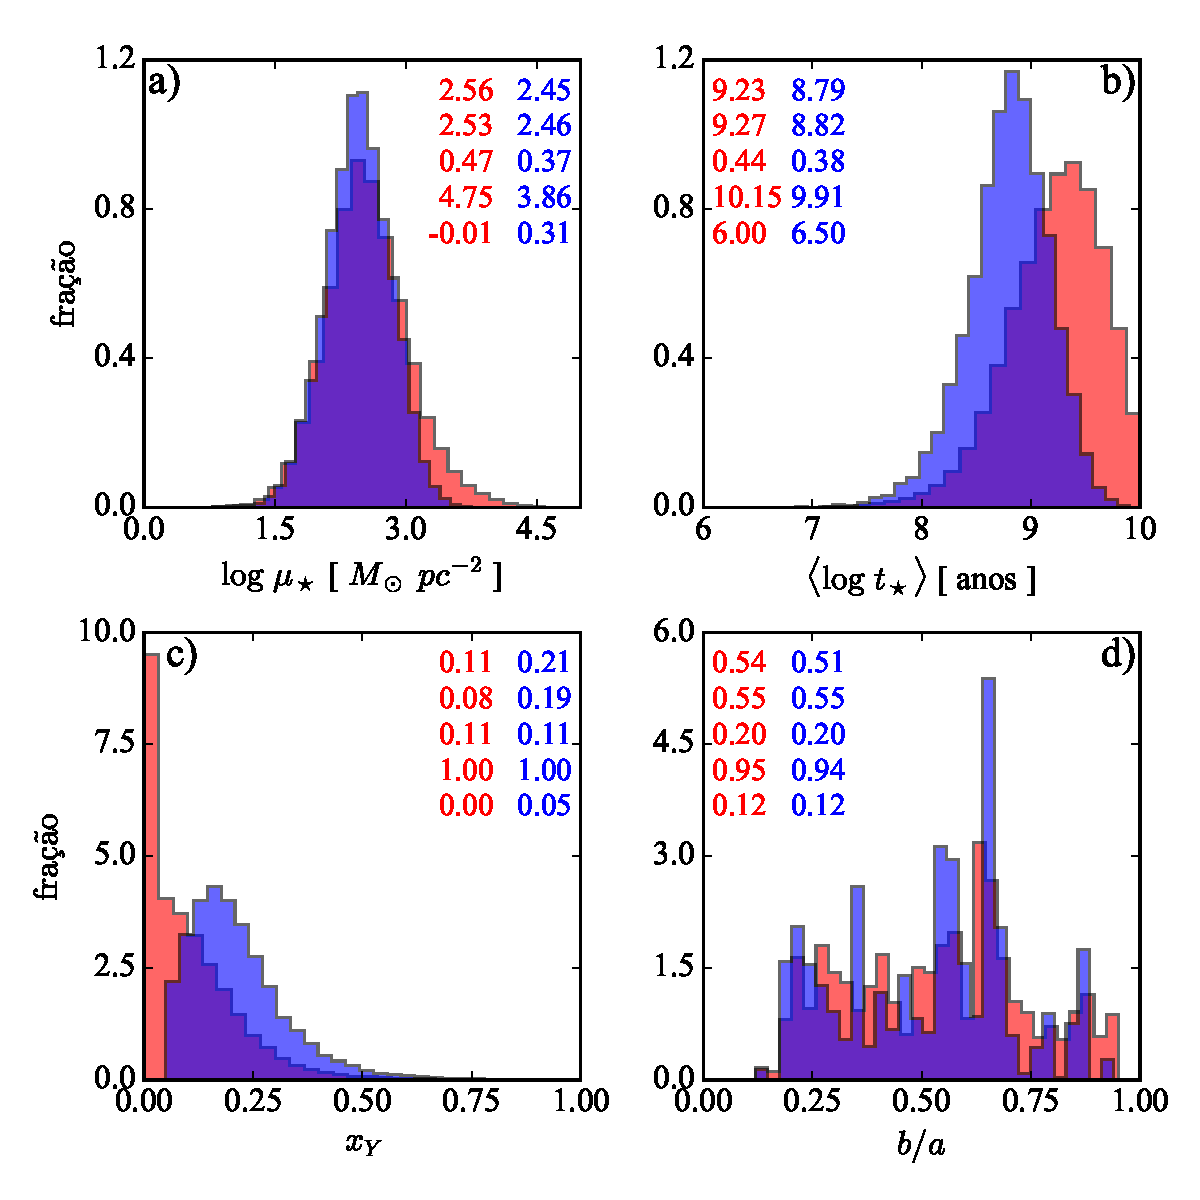
\includegraphics[width=0.99\textwidth]{figuras/histosample.pdf}
	\caption[Histogramas: densidade superficial de massa, idade média, fração de populações jovens e
	relação axial.]
	{Histogramas da densidade superficial de massa ({\em painel a}), idade média das populações estelares ({\em painel b}), fração em luz proveniente de populações jovens ($x_Y \equiv x_Y(t_\star < 31,62$ milhões de anos, {\em painel c}) e relação axial ({\em painel d}). Em vermelho temos a distribuição de valores de 226176 regiões em 305 galáxias e, em azul, a de 16479 zonas de 184 galáxias resultantes após a imposição de algumas restrições. Participam da amostra em azul as zonas em discos ($R > 0,7 HLR$) e onde SN $>3$ nas quatro linhas do BPT (\Hb, \oiii, \Ha, \nii). Em cada gráfico temos os valores da média, mediana, desvio padrão, máximo e mínimo de cada distribuição.}
	\label{fig:histosample}
\end{figure}
%---------------------------- Figure ----------------------------

%Neste apêndice, desenvolvo alguns cálculos de propriedades que estão presentes no módulo \emldc graças às medidas de linhas de emissão,
Realizamos este ensaio para uma amostra do CALIFA com os dados preparados pela {\em pipeline} de redução utilizada no DR2. Começamos com uma amostra de 226176 regiões de 305 galáxias espirais. Nos estudos que envolvem linhas de emissão fixamos um limite SN > 3 para as quatro linhas do BPT (\Hb, \oiii, \Ha, \nii).
%cada linha presente em cada cálculo.
Além dessa censura, mascaramos todas as regiões presentes nos bojos ($R$ > 0,7 HLR) de maneira a nos assegurarmos da influência majoritária de formação estelar em nossas regiões. Ainda dentro dessas limitamos todas as regiões onde não pudemos nos assegurar que 5\% da luz (em 5635 \AA) seja proveniente de populações jovens ($x_Y$). Esse parâmetro é produto da síntese, onde podemos saber qual a fração de luz provém de cada população estelar de diferentes idades e metalicidades.

Na Figura \ref{fig:histosample}, os histogramas normalizados (a integral dentro do intervalo do histograma é 1) de algumas propriedades evidenciam os efeitos da máscara que forma esta amostra. Em vermelho temos as 226176 regiões em 305 galáxias e, em azul, as 16479 zonas de 184 galáxias (19 Sa, 38 Sb, 59 Sbc, 55 Sc e 13 Sd) restantes após a censura dos dados. É notável que nossa seleção busca zonas mais densas e mais jovens (maior fração de populações jovens diminuindo a idade média).
% {\ATR NAO ENTENDI ... }
%
% {\ATR \ojo mais grave: o que isso tudo tem a ver com SK???? tá muito embaralhado!}


\section{Comparação entre as taxas de formação estelar}
\label{apendice:synvsneb:SFR}

O número de fótons que podem excitar \Ha deve ser proporcional a quantidade de estrelas que os produzem (estrelas jovens e massivas). Dessa forma podemos ter uma ideia da taxa recente com que se formam estrelas utilizando a luz que é emitida dessas estrelas mais massivas, dominantes da emissão em \Ha, com escala de tempo de vida bem conhecido ($\sim 10^7$ anos). Utilizando os modelos da síntese podemos calcular teoricamente a relação entre a SFR e a luminosidade de \Ha, $\LHalpha$ (ver Seção \ref{apendice:EMLprops:SFR}). Também com a síntese é possível obter a história de formação estelar, contudo através da fração de populações estelares com distintas idades \citep{Asari.etal.2007a}, não necessitando assim prender-se às zonas das galáxias onde o espectro tenha relação sinal ruído suficiente para a medida de todas as linhas espectrais necessárias para os cálculos sobre o gás e poeira. Uma comparação entre essas duas formas independentes de estimar a mesma propriedade é importante por diversas razões, além de ser um {\em sanity-check} para a síntese. Talvez a mais importante razão seja que calibrando uma parametrização de SFR recente baseado na síntese proporciona a avaliação dessa propriedade em regiões onde a emissão de \Ha não é regida pela a formação estelar e sim por outros regimes de ionização (e.g., AGN, HOLMES).

Para esse cálculo da história de formação estelar através da síntese utilizamos o vetor cumulativo de massa, $\eta_\star(t_\star)$, que integra a fração total de massa convertida em estrelas para cada idade das populações da base ($\mu_j$). Dado um intervalo de tempo $t_\star$, podemos parametrizar a SFR como:
\begin{eqnarray}
	\eta_\star(t_\star)\ &=&\ \sum\limits_{t_{\star,j} > t_\star} \mu_j \\
	\overline{\mathrm{SFR}_\star}(t_\star)\ &=&\ M_\star \frac{(1\ -\ \eta_\star(t_\star))}{t_\star},
	\label{eq:SFRSyn}
\end{eqnarray}
\noindent onde $M_\star$ é a massa total convertida em estrelas durante toda a história de formação estelar de uma galáxia, e a somatória em $\mu_j$ conta apenas as populações da base com idades $t_{\star,j}$ menor que $t_\star$.

\begin{figure}
	\centering
	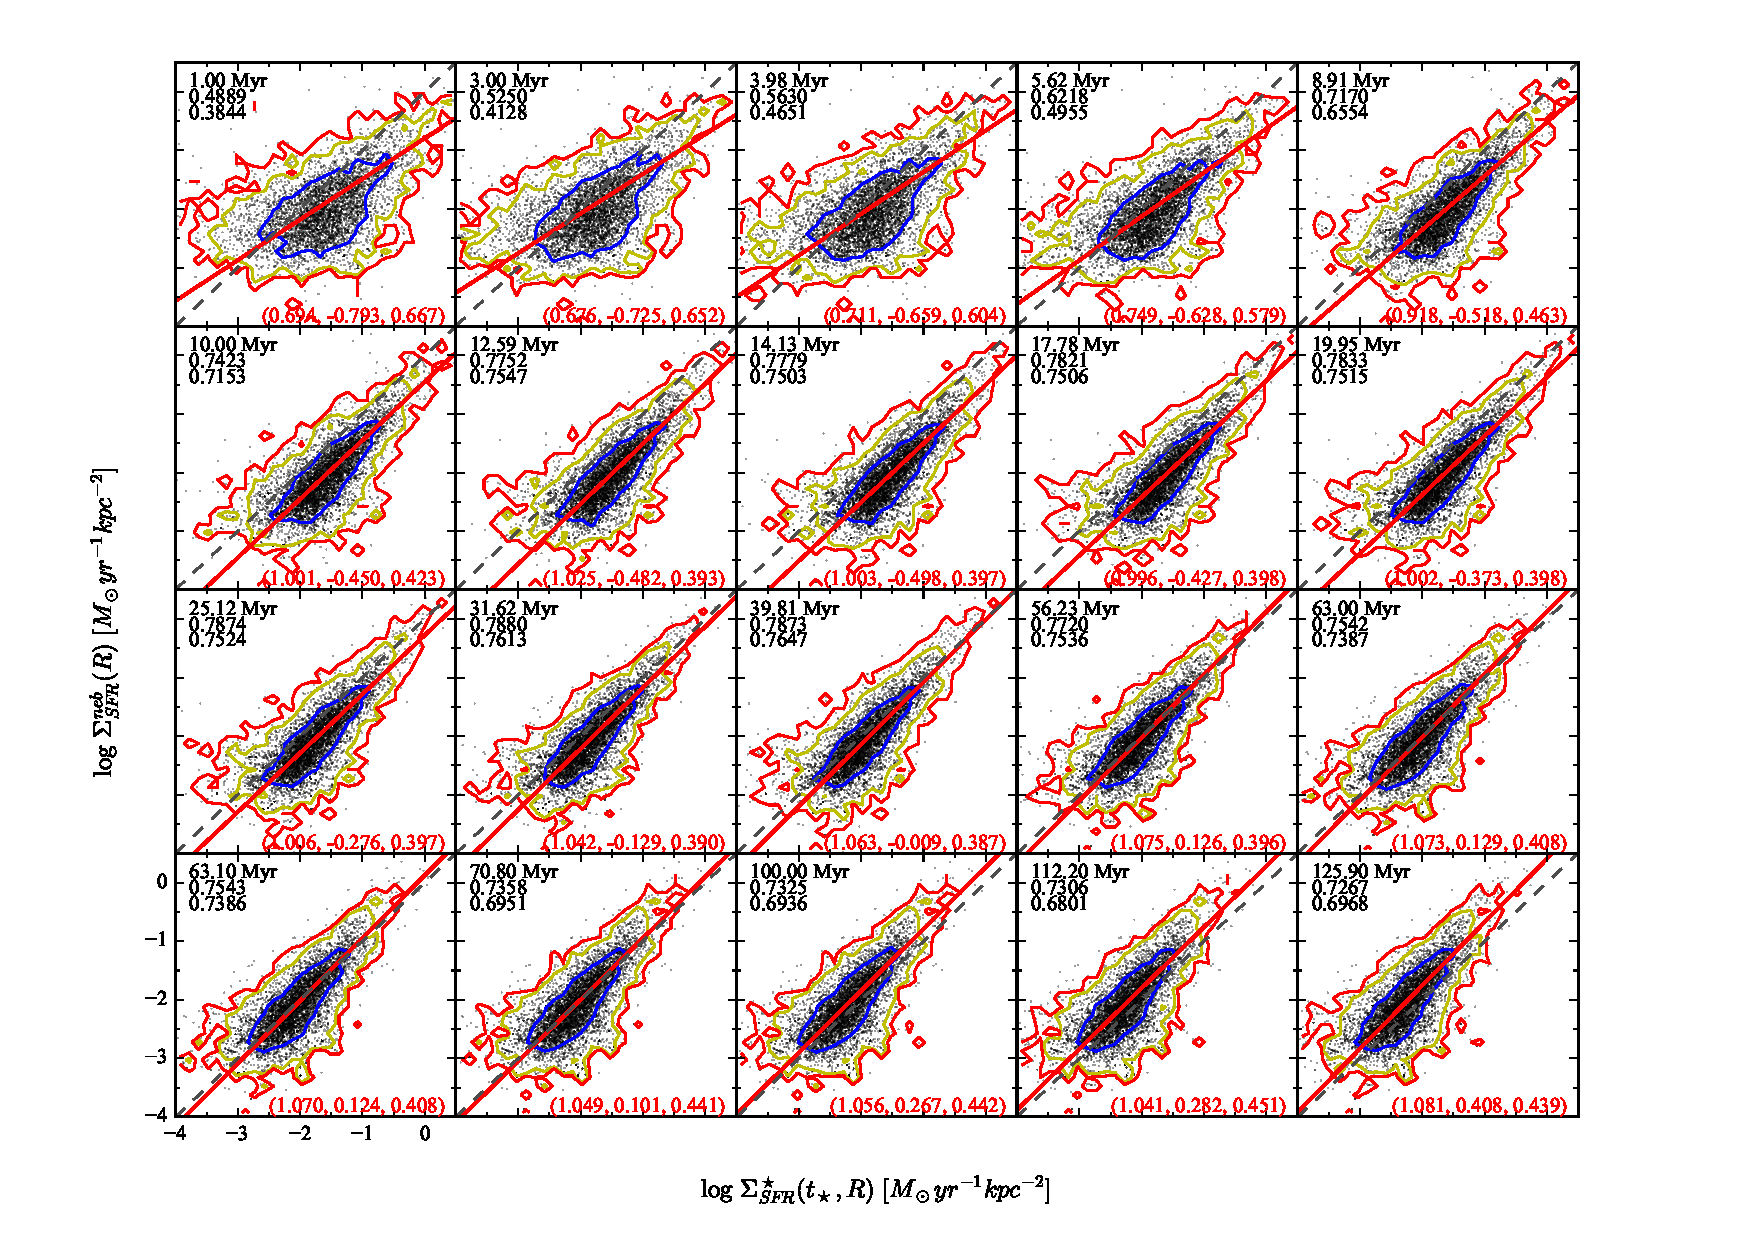
\includegraphics[scale=0.7, clip, angle=90]{figuras/aSFRSD_report.pdf}
	\caption[Comparação entre $\SigmaSFR$ e $\SigmaSFRN$ em {\em bins} radiais para diversas idades]
	{comparação das duas densidades superficiais da taxa de formação estelar em {\em bins} radiais, para diferentes valores de $t_\star$. Em cada gráfico temos os contornos em 1$\sigma$ (azul), 2$\sigma$ (verde) e 3$\sigma$ (vermelho) da distribuição. A linha vermelha indica o ajuste {\em OLS bisector}, e os números em vermelho são o coeficiente angular, o ponto de interceptação com o eixo $x$ e o valor $rms$ em torno do ajuste. No canto superior esquerdo está indicado $t_\star$, o coeficiente de correlação de Spearmann e o de Pearson.}
	\label{fig:aSFRSDsynvsaSFRSDneb}
\end{figure}

Como explicado na Sec. \ref{apendice:EMLprops:SFR}, podemos também medir a taxa de formação estelar recente medindo a luminosidade intrínseca de \Ha. Na figura \ref{fig:aSFRSDsynvsaSFRSDneb} vemos as duas taxas de formação estelar, uma referente às estrelas com idade menor que $\sim 10$ milhões de anos e estimada pela linha de emissão de \Ha (Equação \ref{eq:SFRNeb}), outra proveniente da síntese de populações estelares, que pode ser avaliada em diferentes tempos $t_\star$, modelada pela Equação \ref{eq:SFRSyn}. Essa calibração entre as taxas de formação estelar procura encontrar a idade que melhor relaciona as duas medidas ($t_{\rm SF}$, relativo à {\em star-forming}). Em todos os painéis vemos a comparação das duas densidades superficiais da taxa de formação estelar para diferentes valores de $t_\star$, além de um ajuste {\em OLS bisector} e os coeficiente de correlação de Spearmann e Pearson (números abaixo da idade no canto superior esquerdo). Os pontos representam médias azimutais em cada galáxia (bins em forma de anéis elipticos concêntricos de espessura 0,1 HLR). Vemos que entre 12 e 56 milhões de anos o coeficiente de correlação quase não muda, chegando ao máximo (0,7880) em 31,62 milhões de anos, e por isso escolhemos este valor como $t_{\rm SF}$. Este tipo de análise utilizando as correlações entre densidades superficiais são mais confiáveis já que removem o termo $d^2$ existente no cálculo da SFR, que induz uma correlação indireta entre $\mathrm{SFR}_\star$ e $\mathrm{SFR}_{\Ha}$. De fato o valor de $t_{\rm SF}$ não está muito distante da escala de tempo de vida das estrelas que produzem a maioria dos fótons capazes de produzirem a linha de \Ha ($\sim10^7$ anos).

Esse estudo fez parte da pesquisa publicada no artigo \citep{GonzalezDelgado.etal.2016a} onde nosso grupo analisou as estruturas radiais de $\Sigma_{\rm SFR}$ em uma amostra de 416 galáxias do CALIFA, mostrando que as galáxias espirais possuem $\Sigma_{\rm SFR}$ basicamente constante com uma dispersão pequena. Anteriomente, tal procedimento de comparação foi feito por \citet{Asari.etal.2007a}, no qual os autores encontraram $t_{\rm SF}$ igual a 25 milhões de anos, para 82302 galáxias do \SDSS. A síntese de populações estelares foi realizada utilizando o \starlight, mas com uma diferente IMF. Apesar dessa diferença a concordância entre os resultados é boa. Além de figurar nesse artigo, esse estudo serviu de comparação nos artigos \citet{CortijoFerrero.etal.2017a, CortijoFerrero.etal.2017b, CortijoFerrero.etal.2017c} que dissecaram a história de formação estelar de diversos objetos em interação.

% \begin{figure}
% 	\centering
% 	\includegraphics[scale=0.7, clip]{figuras/Rs_allSFR_cuts.pdf}
% 	\caption[Comparação entre as SFR após cortes]
% 	{Igual a Figura \ref{fig:SFRsynvsneb} mas com a aplicação dos cortes definidos em
% 	\ref{sec:amostra:mask}.}
% 	\label{fig:SFRsynvsneb_cuts}
% \end{figure}
% Figuras:
% - melhor comparação e ajuste

\section{Comparação entre os coeficientes de extinção}
\label{apendice:synvsneb:tauv}

\begin{figure}
	\centering
	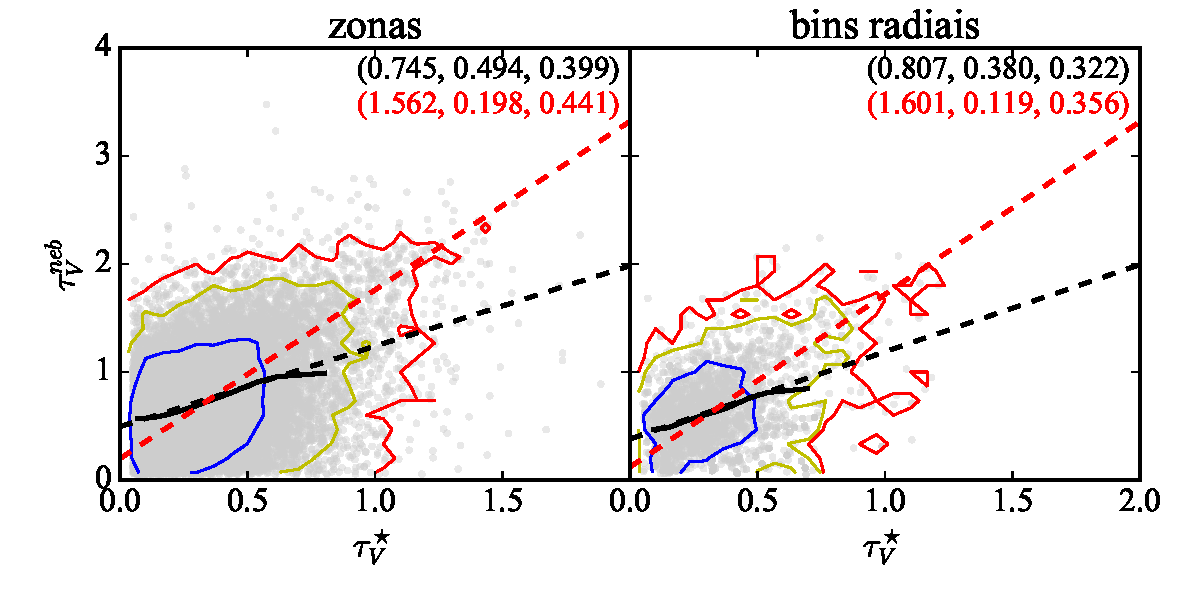
\includegraphics[width=0.99\textwidth]{figuras/CompareTauV_realsample.pdf}
%	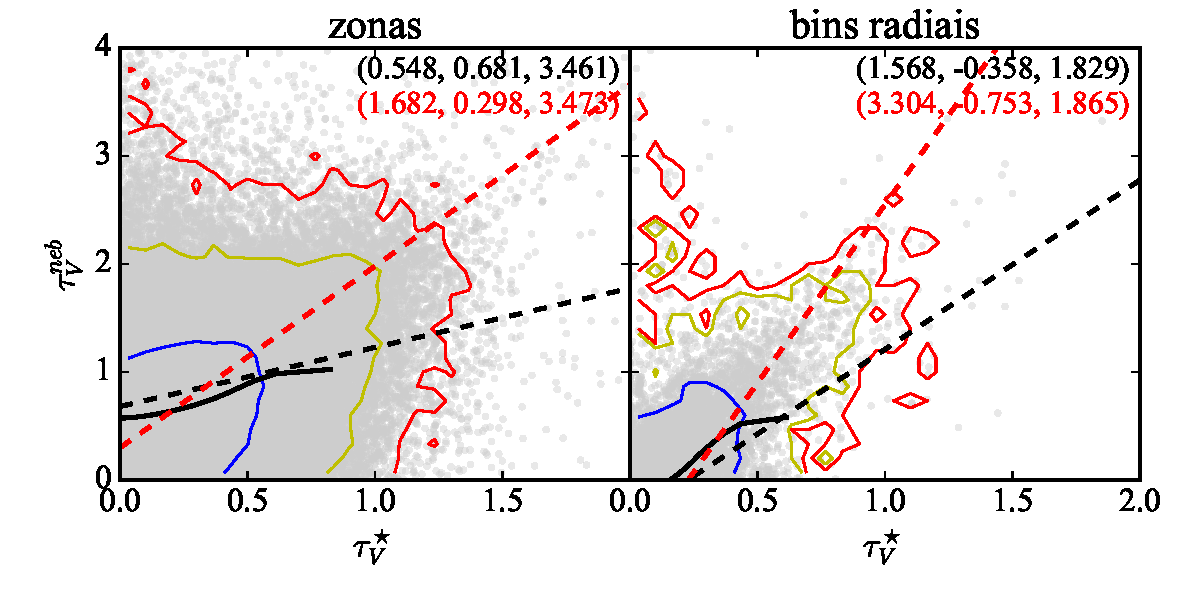
\includegraphics[width=0.99\textwidth]{figuras/CompareTauV.pdf}
	\caption[Comparação entre os coeficientes de extinção]
	{Comparação entre os coeficientes de extinção por poeira provenientes da síntese ($\tauVS$) e do decremento de Balmer ($\tauVN$). Os contornos azul, amarelo e vermelho representam os intervalos de confiança ($1\sigma$, $2\sigma$ e $3\sigma$). A linha preta representa a mediana e as linhas pontilhadas representam o ajuste utilizando {\em OLS bisector} (vermelha) e mínimos quadrados (preta). Como em todos os gráficos com ajustes lineares, em detalhe temos o coeficiente angular, a interceptação da reta com o eixo vertical, e a média quadráticas dos desvios em relação a cada ajuste.}
	% Este gráfico não possui a máscara da definição da amostra aplicada.}
	\label{fig:tauVsynvsneb}
\end{figure}

% \begin{figure}
% 	\centering
% 	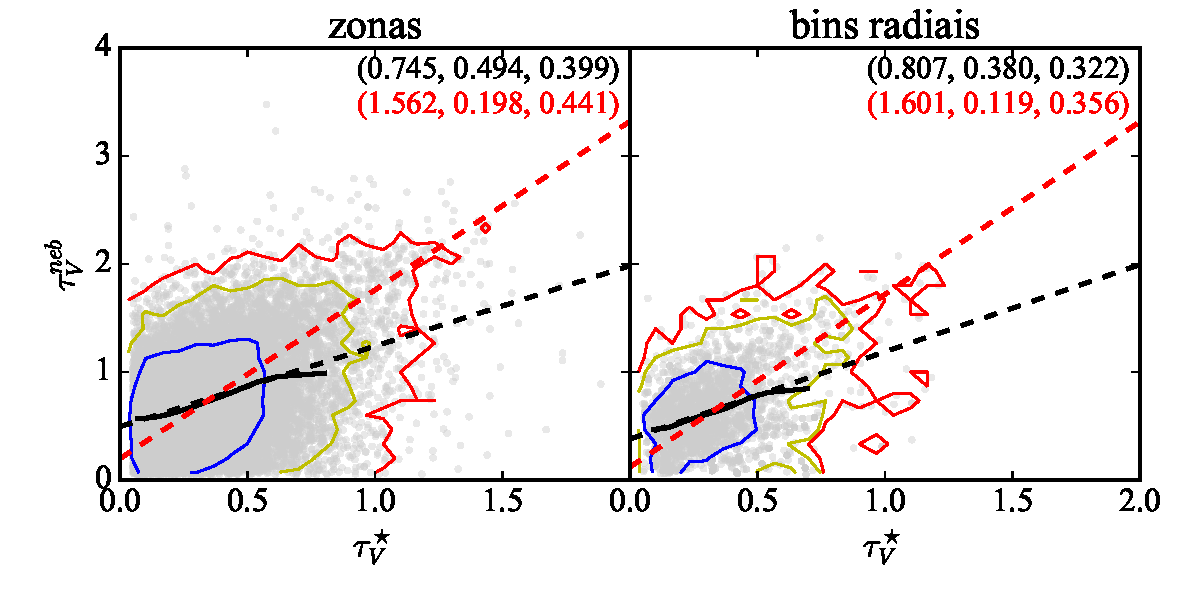
\includegraphics[width=0.99\textwidth]{figuras/CompareTauV_realsample.pdf}
% 	\caption[Comparação entre os coeficientes de extinção da amostra selecionada]
% 	{Igual a Figura \ref{fig:tauVsynvsneb} mas com a aplicação dos cortes definidos em \ref{apendice:EmLinesDataCube:EMLDC:ensaio}.}
% 	\label{fig:tauVsynvsnebMask}
% \end{figure}

A síntese de populações estelares realizadas pelo \starlight adota o mesmo modelo de extinção por poeira explicado em \ref{apendice:EMLprops:tauvneb}, onde todas as populações são atenuadas pelo mesmo fator $e^{-\tau_\lambda}$. Essa simplificação contraria tanto evidências observacionais quanto estudos teóricos, que caminham para um cenário onde populações mais jovens são mais atenuadas pela poeira que populações mais velhas. \citet{Calzetti.etal.1994a} encontraram evidências diretas de que a extinção em regiões \Hii é aproximadamente duas vezes maior do que a das estrelas ($\tauVS \sim 0,44 \tauVN$). \citet{Charlot.Fall.2000a} propõem um modelo onde populações jovens são atenuadas por poeira na núvem de gás que a gerou e encontram que o coeficiente de extinção das {\em birth-clouds} (BC) é cerca de 3 vezes maior que  do meio interestelar (ISM). \citet{Kreckel.etal.2013a} através de dados de espectrografia de campo integrado do KINGFISH \citep{Kennicutt.etal.2011a} calculam a densidade superficial de poeira dessas galáxias e chegam a conclusão que o coeficiente de extinção derivados do contínuo estelar não correlaciona com a quantidade total de massa de poeira, diferentemente daquele derivado do decremento Balmer.

Apesar do modelo de extinção ser o mesmo, o coeficiente calculado por cada um dos procedimentos é diferente, como podemos ver através dos resultados da Figura \ref{fig:tauVsynvsneb} contendo as 16479 zonas que passaram pela máscara imposta e descrita na Seção \ref{apendice:synvsneb:ensaio}. Essa figura apresenta a comparação entre os coeficientes de extinção para zonas e também para os perfis radiais. $\tauVS$, proveniente do \starlight, é calculado no processo de ajuste espectral, já $\tauVN$ só pode ser medido onde existam os observáveis necessários para seu cálculo. Apesar do espalhamento, resulta que $\tauVS$ e $\tauVN$ se correlacionam e a extinção de Balmer se mantém $\sim 2$ vezes maior que aquela proveniente do contínuo estelar. Trabalhos anteriores mostram essa correlação para espectros integrados de galáxias \citep{Stasinska.etal.2004a, CidFernandes.etal.2005a, Asari.etal.2007a}.

\begin{figure}
	\centering
	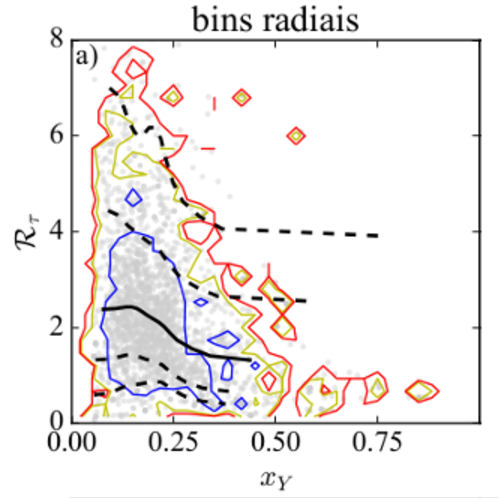
\includegraphics{figuras/RtauVxY.pdf}
	\caption[$\mathcal{R}_\tau \times x_Y$]
	{Relação entre a razão dos coeficientes de extinção nebular (decremento de Balmer) e estelar (modelado pela síntese com o \starlight), $\mathcal{R}_\tau$, e a fração da luz na janela de normalização dos espectros que é proveniente das populações jovens, $x_Y$. No caso utilizamos $t_Y = t_{\rm SF} \equiv 31,62$ milhões de anos. A linha contínua marca a mediana e as tracejadas marcam os intervalos de 1 e 2$\sigma$. }
	\label{fig:RtauVxY}
\end{figure}

Referencio aqui o trabalho de \citet{Mari2016}, que dentre outras comparações, verificou que a razão entre os coeficientes $\tauVN$ e $\tauVS$, $\mathcal{R}_\tau$, se aproxima de 1 quando nos aproximamos de regiões onde a fração de luz proveniente de populações estelares jovens ($x_Y$) é maior. Para nosso estudo espacialmente resolvido o resultado pode ser apreciado na Figura \ref{fig:RtauVxY}. A medida que as regiões são dominadas por populações jovens ($x_Y$ alto) vemos que os coeficientes se aproximam quantitativamente.

Vemos que o cenário de extinção diferencial se confirma e que a medida que vamos para regiões mais com populações estelares mais jovens, o valor da extinção modelada pela síntese se torna semelhante àquele estimado através do decremento de Balmer.

% Figuras:
% - Exemplo de diferenças entre mapas de tau_V
% - comparação entre tauV
% - x_Y

% \section{Comparação entre as metalicidades}
% \label{apendice:synvsneb:Z}
%
% \subsection{Metais em galáxias - \meanM{\log Z_\star} e $\log\ (O/H)$}
% \label{apendice:synvsneb:ZemuZR}
%
% Como citado em \ref{sec:emline:datacube:Zneb}, com a calibração de M13 temos a metalicidade nebular
% para aquelas regiões aonde temos medidas para todas as linhas envolvidas no processo (\Hb, \oIII,
% \Ha e \nII). Já a metalicidade estelar para cada pixel (par $x,y$) é calculada segundo a
% equação:
% \begin{equation}
%  	\label{eq:logZmass}
%  	\langle \log Z_\star \rangle_{M,xy} =
% 	\frac{ \sum_{tZ} M_{\star,tZ,xy} \times \log\ Z}{
% 	\sum_{tZ} M_{\star,tZ,xy} }.
% \end{equation}
% \noindent onde $M_{\star,tZ,xy}$ representa a massa em estrelas com idade $t$ e metalicidade $Z$ no
% pixel $xy$.
%
% Na Figura \ref{fig:compareZR} vemos em detalhe a comparação entre as metalicidades estelar e nebular
% para os perfis radiais e das galáxias de nossa amostra. A comparação entre essas duas propriedades
% deve ser analisada com cuidado, porque estamos tratando de coisas bem diferentes derivadas de
% maneira completamente diferente, todavia a correlação existe e já foi identificada por diversos
% artigos \citep{CidFernandes.etal.2005a, Gallazzi.etal.2005a, CidFernandes.etal.2007a,
% Asari.etal.2007a}. \citet{Stasinska.etal.2006a} enfatiza que esse método de derivação de
% metalicidade nebular utilizando {\em strong-line methods} são calibrados geralmente em gigantes
% regiões \Hii, portanto ainda são necessários estudos sobre os gradientes de metalicidades dentro de
% galáxias. Ainda sim, vejo uma boa correlação entre as duas medidas. Os valores para zonas possuem
% muito espalhamento, mas quando verificamos os valores os perfis radiais (e também os valores
% integrados, embora aqui não demonstrados) vemos que existe uma boa correlação entre as duas com um
% espalhamento pequeno (em todos os {\em bins} menor que 0.2 dex). Vemos também que temos uma
% tendência para que populações na parte mais interna do disco possuam metalicidades mais altas que
% nas partes externas. Essa discussão é muito interessante e precisa ser muito desenvolvida, mas não
% faz parte dessa nossa primeira etapa. Entretanto, a conversão de poeira para gás deve ser dependente
% de metalicidade, portanto, o tema surgirá nas próximas etapas deste trabalho.
%
% \begin{figure}
% 	\centering
% 	\includegraphics[width=0.99\textwidth]{figuras/CompareZR.pdf}
% 	\caption[\meanM{\log Z_\star} vs. $\log\ (O/H)$ - perfis radiais]
% 	{Comparação entre a metalicidade do gás ($\log\ (O/H)$) e metalicidade média das populações
% estelares (\meanM{\log Z_\star}) calculada para diferentes intervalos de tempo (1, 2, 5, 8, 11.3 e
% 14.2 bilhões de anos). Em cada gráfico em vermelho o {\em OLS bisector} e a bissetriz em negro.
% Novamente em detalhe o coeficiente angular, a interceptação da reta com o eixo vertical, e a média
% quadráticas dos desvios em relação ao ajuste.}
% 	\label{fig:compareZR}
% \end{figure}
%
% % \begin{figure}
% % 	\centering
% % 	\includegraphics[width=0.99\textwidth]{figuras/CompareZint.pdf}
% % 	\caption[\meanM{\log Z_\star} vs $\log\ (O/H)$ - galáxias integradas]
% % 	{Igual a Figura \ref{fig:compareZR} mas com um ponto por galáxia (valores integrados).}
% % 	\label{fig:compareZint}
% % \end{figure}
%
% \subsection{Artigo - Insights on the Stellar Mass-Metallicity Relation from the CALIFA Survey.}
%
% No artigo de \citet{GonzalezDelgado.etal.2014b} (GD14 daqui em diante), cuja versão completa está no
% Apêndice \ref{apendice:GDetal2014b}, analisamos a relação entre massa estelar ($M_\star$ - efeitos
% globais) e a densidade superficial de massa estelar ($\mu_\star$ - efeitos locais) com a
% metalicidade estelar ($\meanM{\log Z_\star}$) de uma amostra de 300 galáxias do CALIFA de todos os
% tipos morfológicos (desde E a Sd). \citet{Tremonti.etal.2004a} investigam a mesma relação, embora
% para a metalicidade do gás ($\ZN$) e apenas para galáxias SF. Essa relação é conhecida como relação
% massa-metalicidade ({\em mass-metallicity relation} - MZR). Verificamos que a MZR estelar é mais
% inclinada e se estende em um intervalo muito maior comparando com aquela utilizando a metalicidade
% do gás pois esta última nos fornece informações sobre o estado atual do gás e a primeira, sobre toda
% a história de formação estelar da galáxia.
%
% \citet{Sanchez.etal.2013a} analisa essa relação para $\sim 3000$ regiões \Hii mapeadas em 150
% galáxias do CALIFA. Comparando nossos resultados com os obtidos por \citeauthor{Sanchez.etal.2013a}
% (Figura 2b em GD14) nestas regiões vemos que eles se distanciam conforme $M_\star$ diminui.
% Após calcularmos a metalicidade estelar considerando apenas populações jovens ($t_\star\ \leq$ 2
% bilhões de anos) vemos que o resultado se aproxima melhor da tendência para as regiões \Hii.
%
% Utilizando nossa amostra, vemos na Figura \ref{fig:ZstarvsZneb} a relação entre a densidade
% superficial de massa estelar e a metalicidade nos três painéis de cima (zonas, anéis elípticos e
% galáxias integradas\footnote{Neste painel utilizamos a massa total da galáxia ao invés da densidade
% superficial}) e, na mesma sequência, temos a comparação entre a metalicidade nebular e estelar. Em
% cada gráfico aparecem as medianas para as metalicidades estelares calculadas para diferentes
% intervalos de idades (de 1 a 14 bilhões de anos) de modo a ilustrar a sequência de evolução química
% inferida a partir da síntese. A figura nos mostra que para mesmos valores de $\mu_\star$ a
% metalicidade estelar é mais alta para as estrelas mais jovens, o que parece ser um resultado
% coerente imaginando que o meio onde as novas estrelas nascem vai enriquecendo quimicamente com o
% passar do tempo, fazendo com que novas estrelas tenham maior metalicidade. A metalicidade nebular
% (marcada com uma linha tracejada preta) parece ser muito menos sensível às regiões mais massivas do
% que a metalicidade estelar. \citet{Zahid.etal.2014a}, analisando galáxias com $z \lesssim 1.6$,
% argumentam que esse achatamento acontece quando $M_\star \gg M_{\mathrm{gas}}$ ($f_{\mathrm{gas}}
% \to 0$; ver Eq. \ref{eq:fgas}), assim a quantidade de oxigênio presa dentro das estrelas ({\em
% lock-up fraction}) de baixa massa é da ordem daquela produzida pelas estrelas de alta massa. Os
% modelos de evolução química evoluíram bastante nos últimos anos \citep[e.g., ][]{Lilly.etal.2013a,
% Peng.Maiolino.2014a, Ascasibar.etal.2015a, Peng.Maiolino.Cochrane.2015a} e esperamos que logo
% tenhamos melhores resultados nessa área. O tema é muito interessante e tem muito ainda a ser
% explorado, principalmente quanto aos efeitos locais, quando analisamos esta relação internamente nas
% galáxias e seus efeitos em parâmetros globais. Sobre o painel abaixo, o que vemos é que a variação
% da metalicidade estelar é muito maior do que a nebular e a correlação entre ambas vai aumentando à
% medida que vamos de zonas para galáxias integradas. O painel inferior central condensa todos os
% painéis da Figura \ref{fig:compareZR}.
%
% \begin{figure}
% 	\centering
% 	\includegraphics[width=0.99\textwidth]{figuras/stellar_muZR_realsample.pdf}
% 	\caption[Relação $\mu$ZR e comparação entre as metalicidades]
% 	{Relação $\mu$ZR para zonas ({\em painel a}), {\em bins} radiais ({\em painel b}) e galáxias
% integradas ({\em painel c}). Os pontos desenhados em cada gráfico representam $\meanM{\log Z_\star}$
% calculado para todas as populações com distintas idades, coloridos pela distância radial (barra de
% cores em HLR). Cada gráfico possui a mediana da distribuição de $\meanM{\log Z_\star}$ para
% diferentes intervalos de população ($t_\star \leq$ 1, 2, 5, 8, 11.3 e 14.2 bilhões de anos), além
% da mediana para $\ZN$ ($\log(O/H)$). Comparação $\meanM{\log Z_\star}$ e
% $\ZN$ seguindo a mesma configuração acima (zonas ({\em painel d}), raio ({\em painel e}) e
% integrados ({\em painel f})) com as medianas por diferentes intervalos de população no cálculo de
% $\meanM{\log Z_\star}$ também. Seguindo o mesmo padrão de cores para as medianas, abaixo de cada
% gráfico vemos o coeficiente de correlação de Spearmann entre $\meanM{\log Z_\star}$ e $\ZN$.}
% 	\label{fig:ZstarvsZneb}
% \end{figure}
%
% \subsection{Artigo - The CALIFA Survey across the Hubble sequence. Spatially resolved stellar
% population properties in galaxies.}
%
% Durante o tempo que estive no IAA tive participação em dois artigos. O segundo deles
% \citep{GonzalezDelgado.etal.2015a} (Apêndice \ref{apendice:GDetal2015a}) é um artigo onde
% resolvemos espacialmente as propriedes estelares baseados na síntese com o \starlight para 300
% galáxias do \CAL entre todos os tipos morfológicos. Verificamos que as galáxias mais massivas são
% mais densas, velhas, mais ricas em metais e menos extinguídas por poeira. Discutimos algumas como as
% propriedades se comportam em partes distintas da galáxia (bojo e disco) e o quanto essas
% propriedades variam quando dividimos em classes de massa, idade e tipo morfológico. Galáxias do tipo
% Sb-Sbc possuem gradientes de \meanM{\log Z_\star} compatíveis com aqueles medidos para a Via Láctea.
% Galáxias tipo Sc possuem gradientes mais planos, nos mostrando que a evolução química do disco
% contribui bastante com a evolução química das galáxias desta classe morfológica. Em uma visão geral,
% concluímos que o processo de parada de formação estelar\footnote{Geralmente conhecido como {\em
% quenching}.} é geralmente independente da massa total da galáxia, enquanto metalicidade e a
% estrutura física da galáxia são influenciadas por processos que são dependentes da massa.
%
% %Estudos recentes apontam valores similares para o tempo de depleção do gás \citep[e.g., ][ver tabela 5 e
% %referências.]{Leroy.etal.2013a}. As galáxias mais massivas completaram seu enriquecimento químico a
% %muitas eras atrás, com a história de formação estelar geralmente aproximanda a um único largo broto
% %de formação estelar. Hoje, as galáxias menos massivas são aquelas que possuem maior atividade de
% %formação estelar. Esse fenômeno é conhecido como {\em Downsizing} \myojo{blue}{REFS?}.
%
% % Quando calculamos a metalicidade média das populações jovens das galáxias, estamos olhando para as
% % populações estelares de galáxias menos massivas, mais jovens e com atividade de formação estelar
% % intensa, portanto com um interva
%
% % Figuras:
% % - comparação entre metalicidades
%
% %% End of this chapter
